\documentclass[11pt]{article}
\usepackage{amsmath,amssymb}
\usepackage{graphics}
\usepackage{graphicx}
\newcommand{\numpy}{{\tt numpy}}    % tt font for numpy

\topmargin -.5in
\textheight 9in
\oddsidemargin -.25in
\evensidemargin -.25in
\textwidth 7in

\begin{document}

% ========== Edit your name here
\author{Daniel López - Heber Orellana - Anderson Peña} \date{\today}
\title{Map 1: Curvas de Bezier}
\maketitle

\medskip

% ========== Begin answering questions here
\begin{enumerate}

\item
Curva de bezier de los puntos de control: $P_0(4,1)$, $P_1(28,48)$, $P_3(50,42)$, $P_4(40,5)$
% ========== Just examples, please delete before submitting 
Grafica:
%\begin{figure}
%%==\includegraphics[scale=25]{grafica1.png}
%\caption{Curva de bezier y puntos}
%\label{fig: grafica1}
%\end{figure}
\begin{equation}
    a^2 + b^2 = c^2.
\end{equation}


\begin{equation}
    \mathbf{A} \mathbf{x} = \mathbf{b}.
\end{equation}

\item
Grafica con segmento de recta $\overline{P_0 P_1}$, $\overline{P_1 P_2}$, $\overline{P_2 P_3}$
% ========== Continue adding items as needed

\item
Demostración de tangente en $P_0$ pasa por $P_1$ y la recta tangente de  $P_3$ pasa por $P_2$

\item 
Demostración con letra \emph{C}
\begin{center}
	\begin{figure}[h!]
		\centering
		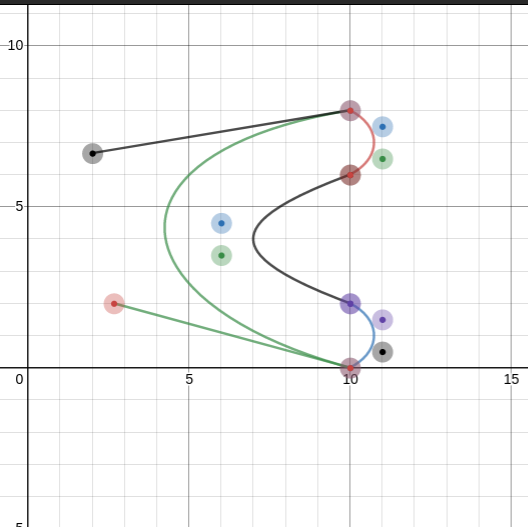
\includegraphics[width=50mm]{LetraCC.png}
	\end{figure}
\end{center}
Ecuaciones que conforman la letra \emph{C}
\begin{equation}
f(x) = 8(1-t)^3 + 20t(1-t)^2 + 6t^2(1-t)+ 0t^3 
\end{equation}
\begin{equation}
f(y) = 10(1-t)^3 + 6t(1-t)^2 + 8t^2(1-t)+ 10t^3 
\end{equation}
\begin{equation}
f(x) = 11(1-t)^3 + 33t(1-t)^2 +33t^2(1-t)+ 10t^3 
\end{equation}
\begin{equation}
f(y) = 9(1-t)^3 + 22.5t(1-t)^2 + 19.5t^2(1-t)+ 6t^3 
\end{equation}
\begin{equation}
f(x) = 10(1-t)^3 + 12t(1-t)^2 + 12t^2(1-t)+ 10t^3 
\end{equation}

Lista de puntos:


\end{enumerate}

\end{document}
\grid
\grid